\chapter{Results }
\section{Motion Segmentation}
We were able to achieve data transmission from the robot with very less latency. We also demonstrated the use of gestures in the virtual reality platform to alter the robot's navigation parameters. A sample video showing this can be found at <give vimeo link here>.
\begin{figure}[h!]
	\begin{center}
		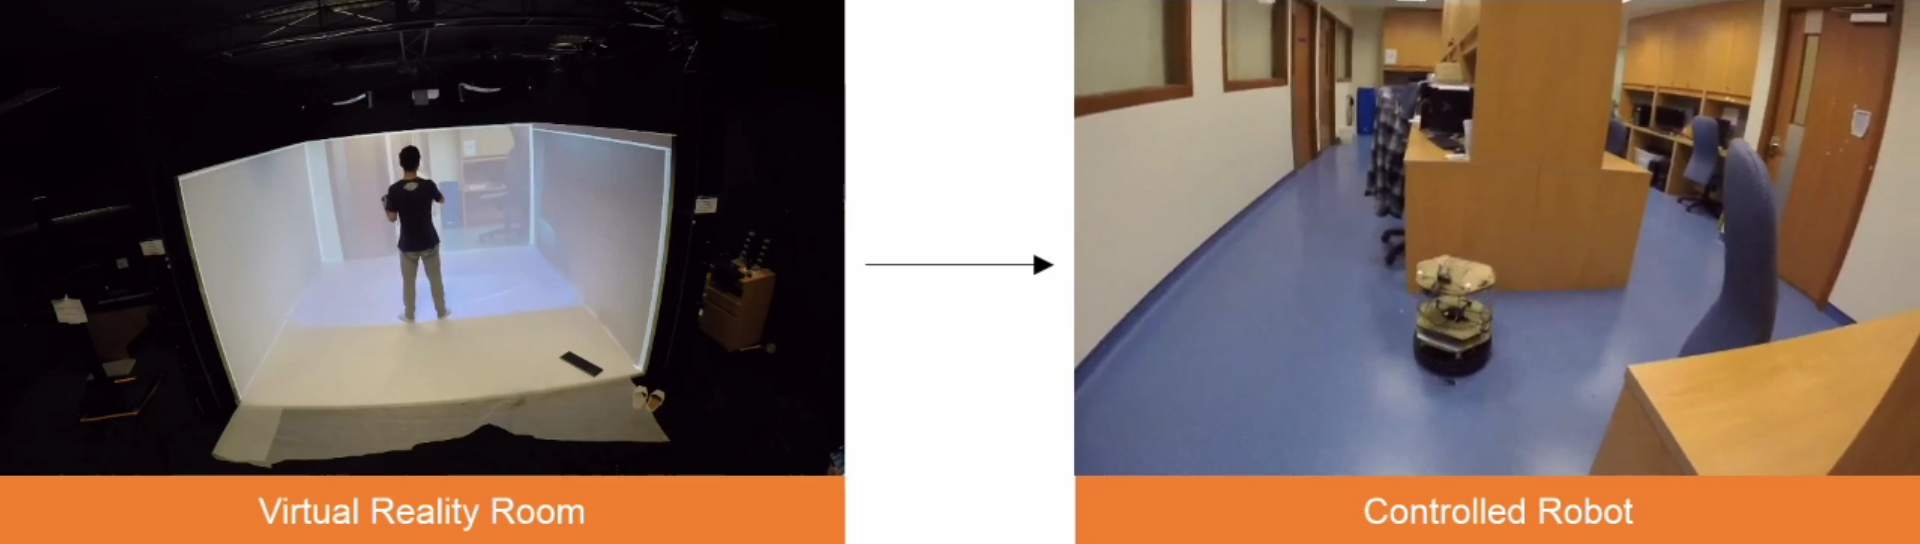
\includegraphics[width=0.99\textwidth]{figures/motion-seg/result}% This is a *.jpg file
	\end{center}
	\textbf{\refstepcounter{figure}\label{fig:result-motion} Figure \arabic{figure}. Real-time robot control and data visualization.} { }
\end{figure}
\section{Vibro-Tactile Haptic Glove}

%%% Local Variables:
%%% mode: latex
%%% TeX-master: "../master"
%%% End:
